% -*- root: These.tex -*-
\graphicspath{{FigureIntroduction/}}

\chapter{Introduction}
\label{sec:Introduction}

\Anotecontent{smil_lund}{Qui donc a pensé à demander à Hägerstrand comment celui-ci avait formulé et programmé pour la première fois son modèle sur l'ordinateur SMIL à Lund ?} %% REF

\Anotecontent{exploration_marge}{Un travail d'exploration rendu possible par l'émergence d'outils pour questionner les marges de ce qui est en train de devenir un nouveau continent numérique dédié au patrimoine scientifique. Ces dernières années ayant vu l'expansion rapide de son volume, principalement du fait de la multiplication des campagnes de numérisation et de la modernisation des métiers et des outils d'archivages.}

\Anotecontent{marble}{Marble a écrit un chapitre dans l'ouvrage de Guetzkow publié en 1972, les deux étant à la même université à cette période, comme celui-ci me l'indique dans un échange privé : \foreignquote{english}{Actually, I was approached by Guetzkow about doing the article. As I recall, he was also on the faculty Northwestern University as I was at that time. }}

\Anotecontent{tobler_review}{\foreignquote{english}{This is a difficult, dangerous, important book. }}

\Anotecontent{guetz}{\foreigntextquote{english}[{\cite[6]{Guetzkow1972}}]{The disadvantages of modeling in general, including simulation, stem from the model's artificiality, abstraction or simplification, and idealization, and the consequent difficulties and dangers in making inferential leaps from a model to the real world. Questions of validity and inference in the model-building process are very important on both theoretical and pragmatic grounds.}}

\Anotecontent{railsback}{Selon \textcite[256]{Railsback2012}⁠, le calibrage des modèles de simulation recoupe trois objectifs : identifier le meilleur ajustement possible avec les données ; trouver les valeurs de paramètres que l'on ne peut pas définir empiriquement, en identifiant les valeurs de façon \enquote{ inverse } dans la recherche d'un meilleur ajustement possible du modèle aux données (\foreignquote{english}{inverse modelling}) ; et la mise en tension de la structure interne du modèle au regard du meilleur ajustement obtenu, ce qui rentre dans la catégorie des tests de robustesse.}

Ce projet de thèse s'inscrit dans la continuité d'un travail de stage initié au laboratoire Géographie-cités en 2009, sous la direction de Thomas Louail et Denise Pumain. C'est de ce moment là que date pour moi la découverte et l'apprentissage passionnants de la modélisation multi-agents, principalement au contact de la famille de modèles Simpop (Simpop1, Simpop2, Eurosim, SimpopNano). Ce projet démarré au début des années 1990 propose d'exemplifier sur différents territoires et pour différentes temporalités les principes d'une \enquote{ théorie évolutionnaire urbaine } \autocite{Pumain1997}.⁠⁠ 

Après quelques mois passés sur l'amélioration du modèle Simpop2, les problématiques déjà soulevées par les précédentes explorations du modèle par Thomas Louail et Clara Schmitt sont apparues clairement. La principale difficulté consiste à l’évaluation des modèles. Avec Thomas Louail nous avons formulé une première réponse à ces problèmes sous la forme d'un projet de plateforme géomatique pour l'automatisation et le partage des explorations de modèles. Intégrée comme un chapitre de perspective dans la thèse de Thomas Louail, cette proposition également reprise dans mon stage de fin d'étude se concrétise dans un projet de thèse financé à la fin de l'année 2009 \autocite{Rey2009} par le réseau R2DS (Réseau Francilien de Recherche sur le Développement Soutenable -un des domaines d’intérêt majeur de la Région Ile-de-France).

A ce même moment, Clara Schmitt, alors ingénieure agronome et titulaire d'un Master 2 recherche en géographie, commence également sa thèse en géographie. Nos deux projets sont conçus en partie de façon interdépendante. Clara propose dans son projet de thèse la réalisation d'un ensemble de modèles (SimpopLocal, SimpopNet, SimpopClim) pour évaluer la dynamique de systèmes de peuplements sous contrainte environnementale à différentes périodes de transitions \autocite{Schmitt2014}⁠. ⁠Mon projet de thèse se construit de façon assez naturelle en parallèle de la création l'un de ces nouveaux modèles (SimpopLocal), car la plateforme a besoin pour exister d'être instanciée au travers d'un cas d'utilisation. C'est ainsi que démarre cette expérience, avec mon inscription active dans la conception, la construction et l'exploration de ce modèle SimpopLocal au sein d'une petite équipe interdisciplinaire (Arnaud Banos, Clara Schmitt, Denise Pumain). Beaucoup de choses vont changer au cours des années qui suivent, avec le rapprochement dès 2010 de notre équipe avec un autre projet de plateforme (OpenMOLE) mené à l'Institut des Systèmes Complexes de Paris Ile-de-France (ISC-PIF), puis l'obtention en 2011 d'une bourse de l’ERC par Denise Pumain. Nous aurons l'ocasion de revenir en détails sur la nature de ces changements dans la partie 2 de cette thèse.

L’extrait de texte suivant, tiré de l'introduction d'un article de Amblard \autocite{Amblard2006},⁠ résume très bien cette situation imaginée, redoutée, et parfois vécue par toute une génération de modélisateurs évoluant au laboratoire Géographie-cités : 

\blockquote[\cite{Amblard2006}]{Une critique récurrente faite aux modèles multi-agents porte sur leur \enquote{ validation }. Il est ainsi fréquent, lors de l'exposé d'un modèle, que la question de la validation, qui se veut être la question piège dans ce domaine, soit posée, plongeant le conférencier dans un embarras bien visible.}

Avec une problématique de thèse axée sur la construction et l'évaluation des modèles, j’ai été amené très vite à explorer les multiples fondations de cette \enquote{ problématique de la Validation } pour mieux tenter d'en extraire les implications. Mais pour déméler les fils complexes de cette question (qu'est ce que la Validation?), et tenter d'en concevoir une réponse plus ancrée dans une discipline géographique qui n'est pas sans \enquote{ histoire }, il faudrait rendre compte de toute la volonté et l'expertise cumulées d'une équipe interdisciplinaire sur plusieurs années. Sans vouloir me substituer à cette voix commune, je propose d'aborder ici les tenants et les aboutissants d'une aventure en deux parties, entre théorie et pratique.

La première partie de cette thèse propose une lecture historique et théorique des problématiques posées par la question de la \enquote{ Validation } des modèles de simulation. Cette réflexion préalable s'est nourrie et développée au fil des années à l'interface de questions méthodologiques et informatiques posées de façon plus immédiate par la réalisation et l'évaluation nécessaires d'un modèle de simulation construit dans un contexte interdisciplinaire (SimpopLocal \autocite{Schmitt2015}). La seconde grande partie souligne ce point de vue plus \foreignquote{english}{ bottom-up } et les besoins de plateformes et d'intégrations qui en découlent, tout en replaçant ce travail et ces problématiques dans l'histoire plus globale d'une évolution des pratiques de modélisation en géographie. La conclusion propose une lecture critique des méthodologies existantes, aiguillée par les apprentissages méthodologiques et techniques qui résultent d’un suivi \enquote{ en temps réel } d’une littérature scientifique en évolution extrêmement rapide.  

\paragraph*{Une construction qui s’appuie sur une histoire de la modélisation}

Les sciences humaines et sociales s'inscrivent dans une tradition d'utilisation de l'informatique et de la simulation vieille de presque 60 ans, qui a produit des outils dont on oublie souvent qu'ils ont pu faire la une des journaux à cette époque, fascinant alors tout autant les sciences physiques que les sciences humaines. Or c'est une histoire pour laquelle il n'existe souvent que des témoignages assez concis sur les aspects techniques \Anote{smil_lund} et des synthèses partielles, abordées sous une perspective linéaire qui ne tient pas forcément compte de l'aspect cumulatif de ces développements techniques (voir le schéma de \autocite{Troitzsch1997} sur la figure \ref{fig:S_Troitzsch})⁠, ou restreintes à une seule discipline, par exemple en archéologie \autocite{Lake2013}, en géographie \autocite{Sanders2013}, ou en sociologie \autocite{Manzo2007}. La tâche pour traiter en détail un front aussi large de contributions sur une période aussi longue que 60 ans est évidemment difficile, voire impossible. Mais il m'a paru intéressant de rappeler de façon moins détaillée, mais sur une portée plus large, toute la diversité de ces premiers travaux de simulation en sciences humaines et sociales \Anote{exploration_marge}.

\begin{figure}[h]
\begin{sidecaption}[Développement des approches contemporaines de la simulation pour les sciences sociales]{ Développement des approches contemporaines de la simulation pour les sciences sociales selon \textcite{Troitzsch1997}}[fig:S_Troitzsch]
 \centering
 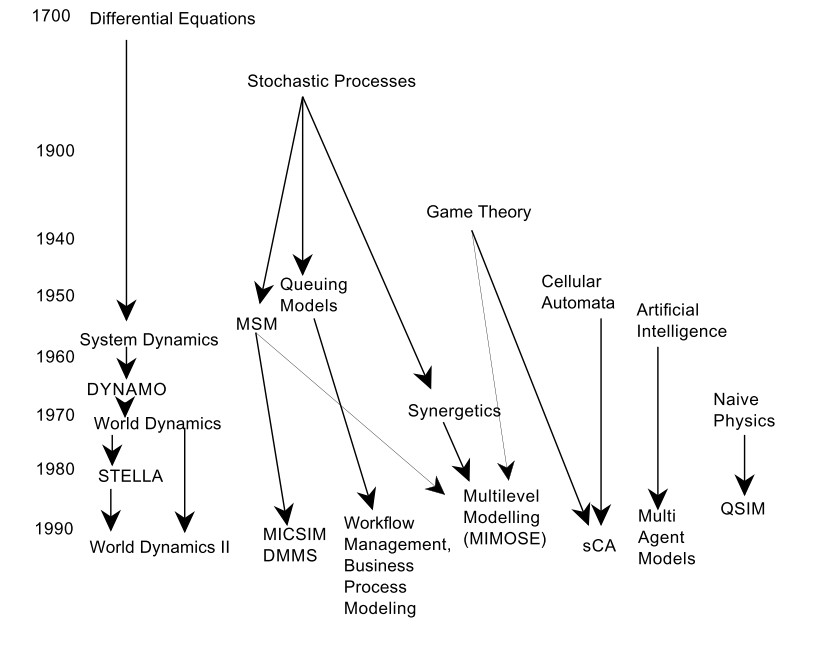
\includegraphics[width=.9\linewidth]{lineaire_figure.jpg}
  \end{sidecaption}
\end{figure}

Cette plongée à rebours dans l'histoire des pratiques de la simulation permet entre autres choses de constater l'ancienneté et la diversité des langages dédiés à la simulation (SIMSCRIPT, GPSS, DYNAMO, SIMULA, etc.), l'existence d'ouvrages et de conférences interdisciplinaires abordant très tôt les différents usages et problématiques soulevés par l'emploi de la simulation dans les sciences humaines et sociales \autocites{Shubik1960b,Shubik1960a, Borko1962, Guetzkow1962, Beshers1965, Guetzkow1972, Shubik1972, Morgan2004, Dutton1971}⁠⁠, et de saisir aussi l'importance des travaux des géographes informaticiens pionniers opérant dans ce contexte comme Marble \Anote{marble}, Pitts, Tobler, Tomlinson, Dacey, etc. \autocites{Marble2010, Marble1972}

Comme souvent pour les effets de mode, cette découverte de la simulation s'accompagne d'un certain emballement dans les usages et les promesses de résultats accompagnant l'usage de ces outils. On connaît bien par exemple les dégâts qu'ont pu faire dans cette discipline les promesses extravagantes sur la simulation et l'intelligence artificielle (\foreignquote{english}{ AI Winter }) (Crevier, 1993). %REF
Cet engouement initial pour les modèles (simulés ou non) sera donc pour certaines disciplines suivi d'une désaffection parfois renforcée par l'émergence de mouvements plus ou moins radicaux dénonçant, entre autre, le coût et la complexité des modèles de simulation construits, l'absence de modèles implémentés ou de résultats, la stérilité et/ou le réductionnisme d'une formalisation mathématique ou informatique trop simplifiante, les problèmes de sous-détermination ou d'équifinalité, voire en géographie l'aliénation philosophique et idéologique de ces nouveaux outils, pour n'en citer que quelques-uns. La géographie quantitative anglo-saxonne n'échappe pas à ces critiques dans le courant des années 1970, et voit même certains des plus proches défenseurs de la modélisation basculer dans l'opposition radicale, comme David Harvey par exemple.

Un certain nombre de ces critiques se rapportent à des problèmes issus des différentes dimensions institutionnelles, techniques, ou philosophiques prises par la \enquote{ problématique de la Validation }. La même famille d'arguments est toujours utilisée \autocites{Amblard2006, Waldherr2013}⁠ pour critiquer l'usage ou la portée explicative des modèles de simulation réalisés. Pour saisir quels sont les enjeux sous-jacents à cette question de la \enquote{ Validation } des modèles de simulation en géographie, il m'a semblé important de poursuivre et de clarifier ce débat en tenant compte à la fois de cette dimension historique et pluridisciplinaire du terme à travers son utilisation dans le courant de la \enquote{ \textit{Validation \& Verification} }, de la philosophie des sciences, et enfin du point de vue des modélisateurs en sciences humaines et sociales. 

\paragraph*{Le problème de la validation tel qu’amorcé par la cybernétique}

Dans un contexte marqué par l'échec des \foreignquote{english}{large scale models} noté dans les années 1960-1970 \autocite{Lee1973} et à côté du développement et de la diffusion parallèles de la micro-simulation, la construction de modèles urbains semble connaître une transformation qui va de pair avec la diffusion mondiale des premiers cadres d'analyse systémique introduits quelques années auparavant \autocites{Ackerman1963, Harvey1969, Berry1964a, Chorley1962, Haggett1965}⁠. Le modèle de simulation Urban Dynamics de Forrester (Forrester, 1969)⁠%REF
est considéré par de nombreux géographes comme un événement charnière cristallisant cette séparation entre les anciens modèles statiques et aspatiaux et les nouveaux modèles spatio-temporels \enquote{ complexes } \autocites{Batty1976, Batty2005}. Le point de vue de Forrester sur la Validation apporte un certain \enquote{ sang neuf } dans la réflexion sur les modèles urbains \autocite{Lee1973}⁠, car il met l'accent non plus sur la présence et la quantité de données dont il faudrait disposer en amont pour construire des modèles \autocite[355]{Batty1976}⁠ mais sur la viabilité d'une démonstration avant tout basée sur la mise en dynamique d'une structure causale, une vision compatible aussi avec l'établissement de modèles plus parcimonieux. Toutefois, comme le laisse supposer l'introduction de \textcite{Tobler1970a} \Anote{tobler_review} dans sa review du modèle, celui-ci vient surtout, dans les faits stimuler la critique d'une génération de géographes comme Batty ou Wilson ayant déjà pour partie intégré la leçon sur les qualités, mais aussi les défauts de toute cette génération précédente de modèles arrivant des Etats-Unis (Batty, 1971)⁠%REF
. Mais, même faux, les résultats contre-intuitifs portés par ce modèle de simulation démocratisent auprès d'un large public de politiques, de scientifiques et de planificateurs les périls (Berry, 1970)%REF
⁠ associés à la modélisation de ces systèmes complexes.

Il m'a paru intéressant d'articuler les réflexions encore empreintes de cybernétique portées par Forrester sur la \enquote{Validation}, avec celles existantes de façon plus générale dans la littérature à cette période. Par exemple, l'économiste Thomas Naylor ou le spécialiste en sciences politiques Charles F. Hermann \autocites{Naylor1966,Naylor1967, Naylor1969, Hermann1967} sont reconnus \autocites{Nance2002, Balci1986} ⁠pour avoir pris au sérieux cette problématique dès le milieu des années 1960, avec la volonté de garantir une certaine crédibilité dans les usages de cet outil simulation. Les ouvrages collectifs interdisciplinaires \autocites{Guetzkow1972, Dutton1971} \Anote{guetz} abordent d'ailleurs frontalement cette problématique au travers de la construction, ou de l'évaluation des modèles de simulation, et ceux-ci méritent à ce titre d'être réexplorés plus en détails afin d'être correctement cités au regard d'une littérature qui ne dit parfois pas beaucoup plus sur cette question. 

\paragraph*{Une plateforme construite pour tirer parti du calcul intensif}

La seconde partie de cette thèse traite de la réalisation d'une plateforme pour la construction et l'évaluation des modèles de simulation, avant tout guidée par la nécessité d'un accès plus démocratisé au calcul intensif chez les géographes. A l'image d'une science géographique construisant et diffusant ses connaissances de façon cumulative (Pumain, 2003, 2005) %REF
⁠, ce projet ne pouvait pas, il me semble, être abordé sans être replacé dans le fil d'une évolution des outils et des pratiques à la fois en géographie et en particulier au laboratoire Géographie-cités.

Depuis plus de 25 ans et dès le début des années 1980, l'utilisation innovante de ressources de calculs intensifs pour la géographie et la modélisation a été pensée, expérimentée puis théorisée par les géographes de l'école de Leeds (Openshaw and Abrahart, 2000; Openshaw, 1983; Turton I. et al., 1996; Turton and Openshaw, 1998)%REF
⁠. Malgré les efforts de ces derniers pour mettre en avant de façon plus pédagogique (Turton and Openshaw, 1998)%REF
 la faisabilité de ces usages au regard des grandes opérations de normalisation touchant le High Perfomance Computing (HPC) dans les années 1990, cette vision n'a jamais percolé en dehors d'un cercle restreint de géographes aux compétences géo-informatiques très avancées. Il s'agit alors d'identifier quels différents éléments ont pu freiner l'adoption de ce qui aurait pu être aussi en France un usage du calcul intensif se plaçant en continuité logique avec les pratiques des premiers géographes. Car, de façon assez équivalente aux usages rapportés par certains géographes informaticiens américains (Marble, 2010)⁠%REF
 , la plupart des pionniers géographes français sont venus à l'informatique par l'apprentissage difficile de la programmation, un usage répété et complexe de cette ressource dans les centres de calculs, et la mise en place de multiples collaborations interdisciplinaires, seule façon pour eux d'accéder à cette ressource dans les années 1970. Il y a donc eu des pratiques, des connaissances, des collaborations, des lieux associés à ces usages pionniers du calcul, et donc de la simulation, pour la géographie. \textit{La micro-informatique a-t-elle vraiment rendu obsolète la pratique des centres de calculs, ou existe-t-il d'autres raisons ? Que reste-il de ces usages aujourd'hui ?} Sur ce point les historiens géographes spécialistes de cette littérature ne semblent pas encore s'être saisis de cette thématique, même si on en trouve déjà quelques traces dans les derniers travaux sur la question \autocite{Cuyala2014}⁠. La récolte de différents témoignages permettra de donner une première visibilité à ces pratiques, en montrant notamment comment certaines d'entres-elles ont pu malgré tout se pérenniser, en dépit des fortes restructurations qu'a subi le paysage du calcul intensif en France dans les années 1990.

Le calibrage \Anote{railsback} des premiers modèles de simulation récupérés dans les années 1980 par l'équipe PARIS (Pumain et al., 1983, 1989; Sanders, 1984)%REF
⁠ nécessite l'usage d'algorithmes d'optimisation (descente de gradients) qui mobilisent pour leur exécution un usage intensif des ressources HPC alors disponibles. Même si cet essai ne permet pas d'obtenir le résultat escompté, il inscrit dans les pratiques ce besoin fondamental d'explorer les modèles, besoin dont on sait qu'il faudra un jour le combler. 

Le fait que nous nous trouvions dans une situation quasi-similaire presque trente ans plus tard, dans un projet interdisciplinaire mobilisant la construction et l'exploration de nouveaux modèles de simulation au travers d'une plateforme développée par des ingénieurs informaticiens spécialistes du calcul intensif, ne pouvait donc pas résulter du seul hasard, et s'inscrit assez logiquement comme la résurgence d'un besoin d'exploration des modèles plus systématique resté latent jusque là. De même que des logiciels de modélisation ont permis l'émergence de mouvements pour l'autonomie de géographes modélisateurs (Banos, 2013)%REF
⁠, il aura probablement fallu attendre l'émergence de logiciels tel que celui développé par les ingénieurs de l'ISC-PIF (OpenMOLE) pour que puisse se démocratiser dans notre discipline encore faiblement formée à l'informatique l'accès et l'usage à des ressources de calcul High Perfomance Computing (HPC) dont on a pourtant identifié depuis bien longtemps la nécessité. 

Cette contingence heureuse mérite toutefois qu'on s'y attarde un peu plus, ne serait-ce que pour comprendre la forme de cet objet commun ayant précipité ainsi cette collaboration entre deux parties aux objectifs, temporalités, exigences apparemment bien différenciés. 

\paragraph*{Une construction dans un contexte interdisciplinaire}

Les dernières réflexions sur l'interdisciplinarité montrent en effet \autocites{Pumain2005, Chapron2014}⁠ que quelque soit la méthode utilisée pour organiser et s'assurer de la réussite d'une activité de recherche interdisciplinaire, il est nécessaire de déconstruire les concepts et les objets engagés par les différentes disciplines pour que puissent émerger d'un processus de co-construction \autocite{Banos2013}⁠ les nouveaux formalismes, grilles et langages communs, et autres objets partagés à même de supporter, voire de catalyser, des enjeux scientifiques qui dépassent le cadre des disciplines prises isolément.

On aurait tort de penser cette déconstruction opérante sur le seul plan de la vie des idées, les outils étant également impactés, surtout lorsqu'une équipe de géographes est amenée à intégrer les projets d'ingénieurs informaticiens engagés depuis plusieurs années dans la réalisation d'une plateforme aux objectifs autonomes. Suite au constat en 2010 d'une convergence potentielle entre les deux projets, il a fallu pour que la coopération s'avère plus bénéfique encore, savoir se dessaisir d'un projet scientifique et technique conçu pour les besoins des géographes, à l'échelle d'une personne et d'une thèse \autocites{Rey2009, Louail2010}⁠, pour la réinventer au travers de nouveaux objectifs communs, en inter-dépendance avec une équipe d'ingénieurs forte de son propre calendrier et de ses propres objectifs de développement, au contact d'un projet déjà mature et complexe. 

L'insertion de mon travail dans ce processus interdisciplinaire se fait dans le remplacement progressif d'un objet par un autre, à la fois plus prometteur dans les évolutions qu'il propose au-delà du cahier des charges fixé initialement, mais aussi beaucoup moins maitrisé et maitrisable sans faire appel aux compétences de deux ingénieurs évoluant dans des temporalités de développement très différentes, ce qui ne sera pas sans causer certains inconvénients. \textbf{Il ne s'agissait donc plus de créer la plateforme, mais de l'intégrer, en appelant la construction de nouveaux outils et de nouvelles méthodes pour la construction et l'exploration plus systématique des modèles de simulation, dans un projet bénéfique aux deux parties} \autocite{Pumain2014}⁠.

\paragraph*{Les étapes de construction de la plateforme}

L'exploration des modèles de simulation devient l'objet de recherche par lequel transitent les préocupations communes aux deux équipes. Le travail s'organise sur deux fronts dans lesquels je suis inscrit comme développeur, avec la création de SimpopLocal d'une part, et d'autre part la construction parallèle des nouveaux outils à même de supporter l'exploration de celui-ci dans OpenMOLE. Le hasard a fait qu'il existait dans chacune des équipes originales une volonté de traduire l'exploration des modèles de simulation en s'appuyant sur l'utilisation d'algorithmes d'optimisation pris dans la famille des Algorithmes Evolutionnaires. C'est donc en repartant d'un premier framework nommé MGO, développé dans une version encore instable en 2010 à l'ISC-PIF, que cette première intégration de la plateforme prend place.

Entre 2010 et 2013, l'équipe se focalise sur la réalisation d'un premier prototype fonctionnel démontrant la faisabilité d'une exploration plus systématique du modèle de simulation SimpopLocal en utilisant OpenMOLE et MGO. Par extension, et c'est là une des forces de cette collaboration, la méthodologie et les outils développés sont mutualisés au sein d'OpenMOLE et deviennent par extension utilisables pour d'autres modèles de simulation \autocites{Schmitt2014, Reuillon2015} 
 
C'est sur la base de cette exploration systématique appuyée par le HPC et des Algorithmes Evolutionnaires que va se constituer dans notre équipe une nouvelle génération de modèles de simulation et de nouvelles méthodes de construction et d'exploration des modèles (Cottineau, 2014; Cottineau et al., 2015; Chérel, 2013)%REF
⁠. Ces développements se feront aussi en regard des nouvelles possibilités permises par l'usage facilité du HPC (Openshaw and Abrahart, 2000)⁠, mais aussi au travers d'une réflexion commune sur les questions épistémologiques associées à l'usage de ces nouveaux outils. 

J’ai souhaité introduire ce travail en présentant des éléments de contexte qui l’ont fortement contraint et inspiré. La rédaction de la thèse a obéi à deux motivations étroitement enchevêtrées : la première partie expose les cheminements des raisonnements relatifs à la modélisation et à la validation. J’ai mené cette enquête, qui n’était pas exigée par mes encadrants, et pour laquelle je ne disposais pas de formation particulière, pour satisfaire à une exigence intellectuelle ; la méthodologie que j’ai utilisée ne relève donc pas des canons de l’épistémologie ou de l’histoire des sciences, mais d’une remontée approfondie dans l’histoire des sources sur cette question, appuyée sur une bibliographie très abondante et des interrogations par voie écrite ou orale adressées à des acteurs majeurs de ce domaine. La seconde partie retrace la logique de construction et d’intégration d’une plateforme dans une perspective de géographe informaticien, selon des méthodes qui sont entièrement explicitées. La conclusion permet de faire le lien entre cette expérience de réalisation et les problèmes relevés dans la première partie, tout en tentant une évaluation à la lumière des réalisations les plus récentes de ce domaine de recherche très actif. 